%\section*{Collaborators}
%List all your collaborators.

\documentclass[11pt]{article}

\usepackage[margin=1in]{geometry}
\usepackage{amsmath,amsthm,amssymb}
\usepackage{color}
\usepackage{lipsum} % for filler text
\usepackage{fancyhdr}
\pagestyle{fancy}
\usepackage{enumitem}
\usepackage{graphicx}
\usepackage{array}
\usepackage{tabu}

\newenvironment{problem}[2][Problem]{\begin{trivlist}
\item[\hskip \labelsep {\bfseries #1}\hskip \labelsep {\bfseries #2.}]}{\end{trivlist}}

\fancyhead{} % clear all header fields
\renewcommand{\headrulewidth}{0pt} % no line in header area
\fancyfoot{} % clear all footer fields
\newcommand\tab[1][1cm]{\hspace*{#1}}
\fancyfoot[LE,RO]{\thepage}           % page number in "outer" position of footer line
\fancyfoot[RE,LO]{Aashish Dhakal} %your name in footer line

\begin{document}
%\lipsum[1-20]
\title{CS 572(Assignment 8)} %replace X with the appropriate number
\author{Aashish Dhakal\\ %replace with your name
aashish@iastate.edu\\%replace with username
 }      %if necessary, replace with your course title
\date{}


\maketitle
\section*{}

\textbf{Problem 14.1}
\begin{enumerate}[label=(\alph*)]
  \item Let $M$ be the random variable denote which coin of $\{ 1, 2, 3 \}$, where $C=1$ represents that the first coin was drawn from the bag
  and so on. So, we will have the following Bayesian network.
        The Conditional Probabilistic table for $C$ is:\\ \\
        \begin{tabular}{ | m{0.5cm}| m{1.8cm} | }
          \hline
            $C$ &  $P(C=c)$ \\
            \hline
            $1$ & $1/3$ \\
            \hline
            $2$ & $1/3$ \\
            \hline
            $3$ & $1/3$ \\
            \hline
       \end{tabular}\\ \\

    \begin{figure}
        \center
        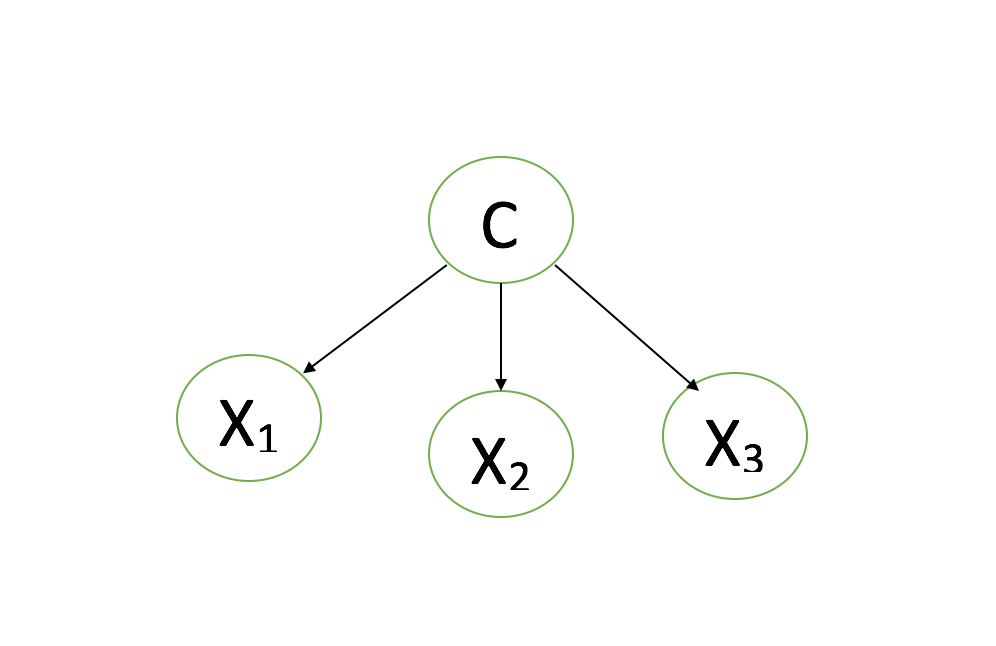
\includegraphics[width=6cm, height=5cm]{bay.png}
          \caption{Bayesian Network}
  \end{figure}

        The CPT for $X_1$ (with C)is:\\ \\
          \begin{tabular}{ | m{0.5cm} | m{1cm}| m{3cm} | }
            \hline
            $X$ & $C$ & $P(X_1=x|C=c)$ \\
            \hline
            $1$ & heads & 0.2 \\
            \hline
            $2$ & heads & 0.4 \\
            \hline
            $3$ & heads & 0.6 \\
            \hline
            $1$ & tails & 0.8 \\
            \hline
            $2$ & tails & 0.6 \\
            \hline
            $3$ & tails & 0.4 \\
            \hline
        \end{tabular}\\ \\
The CPT for $X_2$ and $X_3$ is going to be the same so it's not shown. Here we also assume that coin-flips are independent,
given information about the coin itself. Note also that here variables $X_i$ have domains $\{ h, t\}$, which corresponds to
heads up and tails up.
\item Let’s denote the event that the coin came out “heads” twice and “tails” once by $B$. Then we need to find $i \in \{ 1, 2, 3 \}$
such that $P(C=i|B)$ is maximal. Let’s use Bayes’ rule for that:\\
  \[ P(C=i|B)=\frac{P(B|C=i)P(C=i)}{P(B)} \]\\
Note that:\\ \[ \frac{P(C=i)}{P(B)} \] \\ is constant forall $i \in \{ 1, 2, 3 \}$ (Since, $P(C=i)=1/3$ for all $i$)\\
Therefore, we need to find such $i$ that maximizes $P(B|C=i)$. Assume that probability of “heads up” for a coin $i$ is $Q$.
Then, $P(B|C=i)\; = 3Q^2(1-Q)$ , where 3 is the number of different ways event $B$ might have occurred (i.e., heads-heads-tails,
heads-tails-heads, or tails-heads-heads). Let’s find a max:
\begin{itemize}
  \item For $i = 1:\; 3Q^2(1-Q)\; =\; 3*0.2^2*0.8 = 0.096 $,
  \item For $i = 2:\; 3Q^2(1-Q)\; =\; 3*0.6^2*0.4 = 0.432 $,
  \item For $i = 3:\; 3Q^2(1-Q)\; =\; 3*0.8^2*0.2 = 0.384 $
\end{itemize}
which shows that coin 2 is the most likely one.

% The coin most likely to have been drawn from the bag given this sequence  the value of $C$ with th greater prosterior probablity
% $P(C\;|\; 2 \; heads, \; 1 \; tails)$. Now, \\
% $P(C\;|\; 2 \; heads, \; 1 \; tails)$ = $P(2\; heads, \; 1 tails|C)P(C)/P(2\; heads, \; 1 \; tails)$ \\
% $\propto \; P(2\; heads, \; 1 tails|C)P(C)$ \\
% $\propto \; P(2\; heads, \; 1 tails|C)$\\ \\
% where in the second line we observe that the constant of proportionality $1/P(2\; heads, \; 1 \; tails)$ is independent of $C$, and also for
% last we observe that $P(C)$ is independent of the value of $C$, as by hypothesis it is equal to $1/3$.\\ \\
% From Bayesian network we can see that $M_1, M_2 \; and \; M_3$ are conditionally independent given $C$. For eg:\\
% $P(M_1 \; = \; tails,\; M_2 \; = \; heads,\; M_3 \; = \; heads|C \; = \; a)$\\
% $=\; P(M_1 \; = \; tails|C \; = \; a)P(M_2 \; = \; heads|C \; = \; a)P(M_3 \; = \; heads|C \; = \; a)$\\
% $=\; 0.8 * 0.2 * 0.2 = 0.032$\\
% Since, the CPTs for each coin is same, we would get the same probablility above for any ordering of 2 heads and 1 tails.
% As we have three such orderings, we have:\\
% $P(2heads,\; 1tails|C \; = \; a)\;=\; 3*0.032 \;=\; 0.096$\\
% Similarly,\\
% $P(2heads,\; 1tails|C \; = \; b)\;=\; 0.432$\\
% $P(2heads,\; 1tails|C \; = \; c)\;=\; 0.384$\\
% which means that coin $b$ is likely to be drawn.
\end{enumerate}

\textbf{Problem 14.14}
\begin{enumerate}[label=(\alph*)]
  \item
      \begin{enumerate}
        \item Not asserted, since the network shows that $B, I$ and $M$ are NOT mutually independent: $I$ is dependent on both $B$ and $M$.
        \item This is asserted, since $G$ is the only parent of $J$ and $I$ is not a $J'$s descendant. Therefore, by construction $I(J, G, I)$.
        \item This is also asserted by the separation property: $B$ is separated from $J$ by $\{ I, M, G\}$. Therefore, $I(B,\{ I, M, G\}, J)$.
      \end{enumerate}
  \item Let's apply chain rule:\\
  $P(b, i, \neg m, g, j) = P(j|b, \neg m, g, i)P(b, \neg m, g, i) \\ = P(j|b, \neg m, g, i)P(g|\neg m, b, i)P(\neg m, b, i)
  \\ = P(j|b, \neg m, g, i)P(g|\neg m, b, i)P(i\neg m, b)P(\neg m, b)$\\
  Now using the local independence assumptions, provided by the network:\\
    $P(j|g)P(g|\neg m, b, i)P(i|\neg m, b)P(b)P(m)$\\
  = 0.9 * 0.9 * 0.5 * 0.8 * 0.9 = 0.2916
  \item The goal is to calculate $P(j|b,i,m)$.\\
  We can do that as follows (Bayes’ rule and summing out on $G$):\\
  \[ P(j|b, i, m)=\frac{P(j, b, i, m, g) \; + \; P(j, b, i, m, \neg g)}{P(b, i, m)} \]\\
  We can reuse the chain found in item (b) to calculate the above probability:\\
  $P(j,i,b,m,g)= P(j|g)P(g|m,b,i)P(i|m,b)P(m)P(b)\\
  \; = \; 0.9*0.9*0.9*0.1*0.9=0.06561$\\ \\
  $P(j,i,b,m,\neg g) = \; P(j|\neg g)P(\neg g|m, b, i)P(i|m, b)P(m)P(b) = 0$\\
  $P(b, i, m)= P(i|b,m)P(b)P(m) = 0.9*0.9*0.1=0.081$\\ \\
  As a result,
    \[ P(j|b, i, m)=\frac{P(j, b, i, m, g) \; + \; P(j, b, i, m, \neg g)}{P(b, i, m)}=\textbf{0.81} \]\\ \\
\textbf{Markov Blanket}\\
A Markov blanket for $B$ should include all its parents (none), all its children $(\{ I, G\})$,
and parents of the children $(\{ M\})$. Summing that up, Markov blanket for $B$ consists of \textbf{I, G, M}.


  %
  % Here $B, I, M$ are fixed true in evidence.\\
  % We will just look at the submodel with $G,J$:\\
  % $P(J|b, i, m) = \propto $$\sum_{g} P(J, g)$$ = \propto [P(J, g)\; + P(J, \neg g)]$\\
  % $= \propto [\langle P(j, g),\; P(j, \neg g) \rangle \; + \langle P(j, \neg g),\; P(\neg j, \neg g) \rangle]$\\
  % $= \propto [\langle 0.81, 0.09 \rangle + \langle 0, 0.1 \rangle] $
\end{enumerate}
\end{document}
}
